In the following experiments, we used two motions from the CMU Graphics Lab Motion Capture Database \cite{mocap}. As seen in subsection \ref{subsec:shape-lie}, motion capture data can be interpolated such that the SRV form is piecewise constant. As in the previous section, these SRV curves were then interpolated by a piecewise linear interpolation. The interpolated curves were then used instead of the original curves in the optimization procedure. As seen in Figure \ref{fig:curve_1_so3_example} the interpolated problem produced an in optimal reparametrization that agreed with the solution given by dynamic programming, implemented by \citeauthor{lystad2019}\cite{lystad2019}. 

\begin{figure}[t]
    \begin{subfigure}[t]{0.5\textwidth}
        \centering
        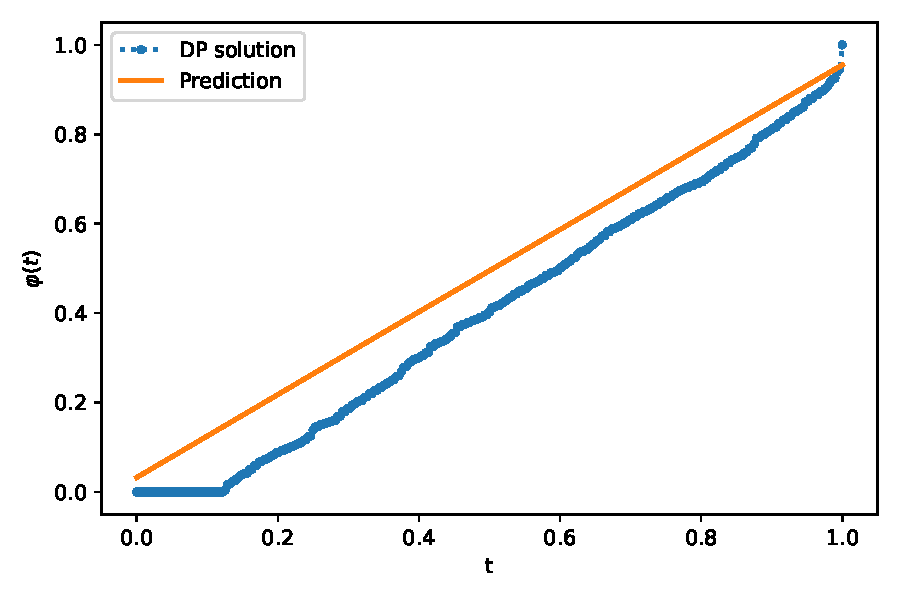
\includegraphics[width=\linewidth]{figures/curve_so3/pc_eks_2/plot_1_0.pdf}
        \caption{Solutions found by neural network training and dynamic programming.}\label{fig:curve_so3_pc_solution}
    \end{subfigure}a
    \begin{subfigure}[t]{0.5\textwidth}
        \centering
        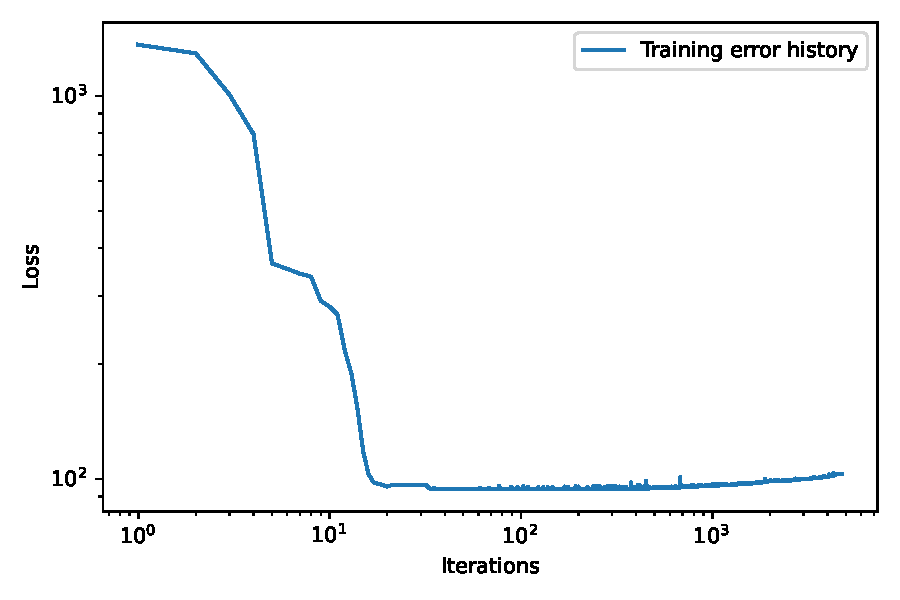
\includegraphics[width=\linewidth]{figures/curve_so3/pc_eks_2/history_plot_1.pdf}
        \caption{The cost function \(L(\theta)\) with each iteration.}\label{fig:curve_so3_pc_history}
    \end{subfigure}
    \begin{subfigure}[t]{0.5\textwidth}
        \centering
        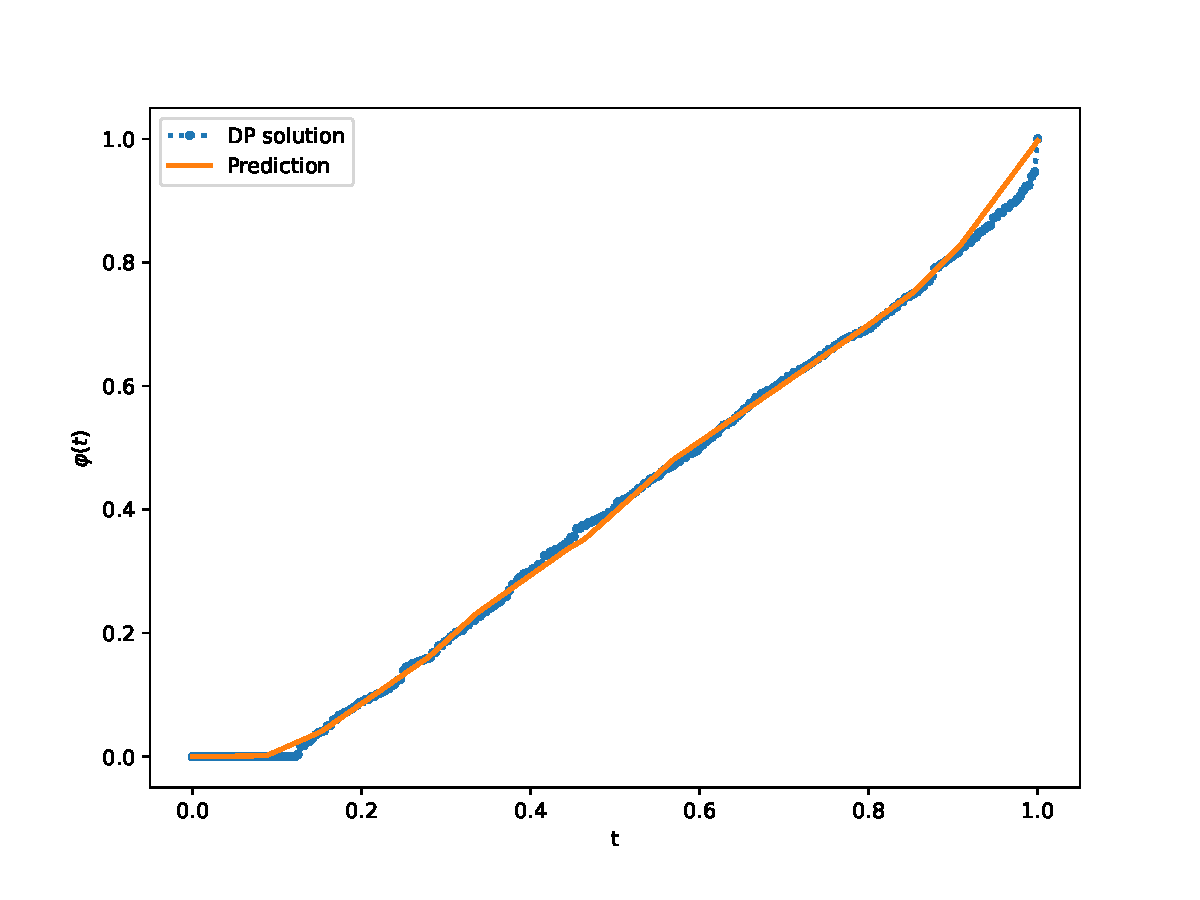
\includegraphics[width=\linewidth]{figures/curve_so3/pl_eks_6/plot_288_0.pdf}
        \caption{Solutions found by neural network training and dynamic programming.}\label{fig:curve_so3_pl_solution}
    \end{subfigure}
    \begin{subfigure}[t]{0.5\textwidth}
        \centering
        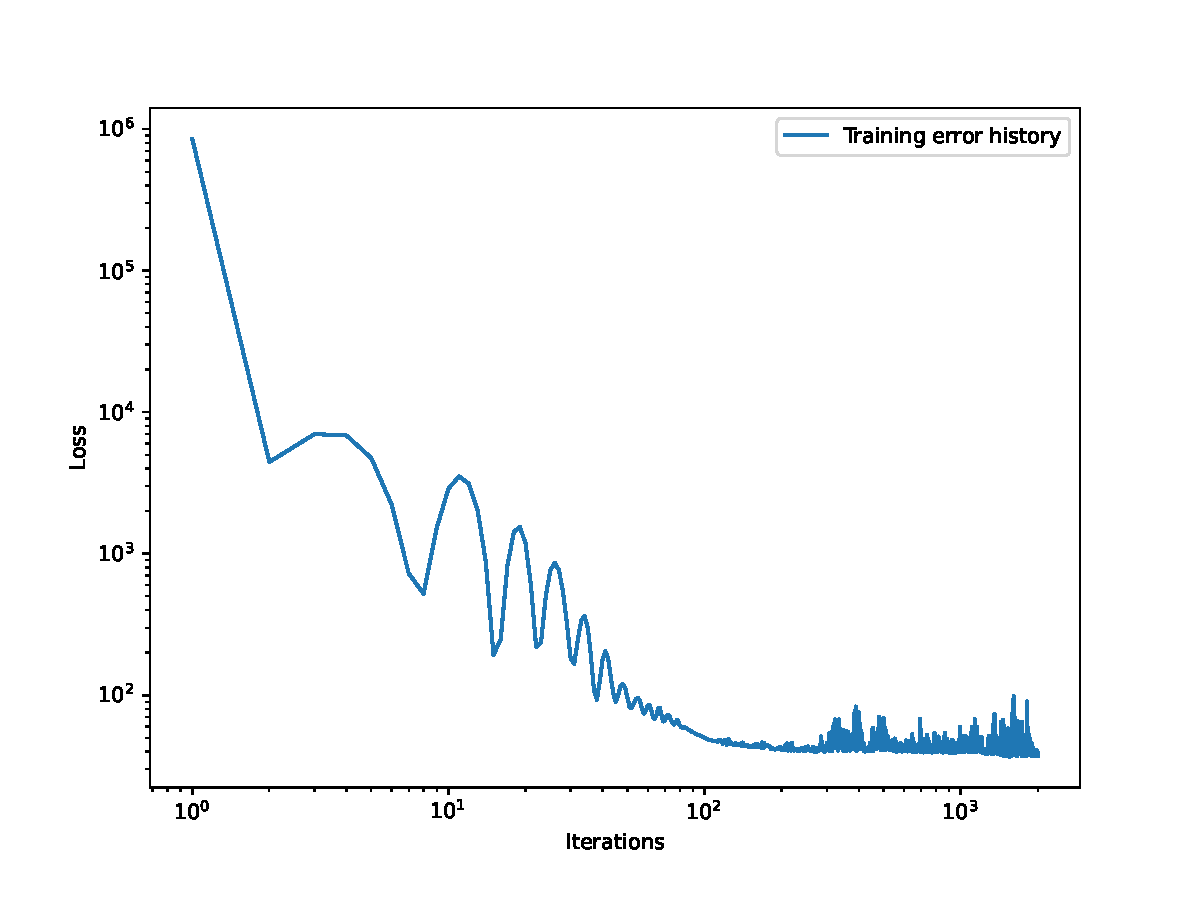
\includegraphics[width=\linewidth]{figures/curve_so3/pl_eks_6/history_plot_288.pdf}
        \caption{The cost function \(L(\theta)\) with each iteration.}\label{fig:curve_so3_pl_history}
    \end{subfigure}
    \caption{The approximate optimal reparametrizations of two curves representing motion capture data. Figure \ref{fig:curve_so3_pc_solution} shows the solution for the original curves, and Figure \ref{fig:curve_so3_pl_solution} shows the solution for the linearly interpolated curve. The approximate solutions are compared to the solution found by a dynamic programming algorithm and the corresponding training history is shown in the figure to the right. }\label{fig:curve_1_so3_example}
\end{figure}

Ensemble training was again performed to observe how the optimal reparametrization is affected by different parameters. The ensemble training result is shown in Figure \ref{fig:curve_so3_pl_eks}. In this experiment, the network structure was not varied. Instead, the performance of ReLU and \(\tanh\) activation function was compared. 

\begin{figure}[t]
    \begin{subfigure}[t]{0.5\textwidth}
        \centering
        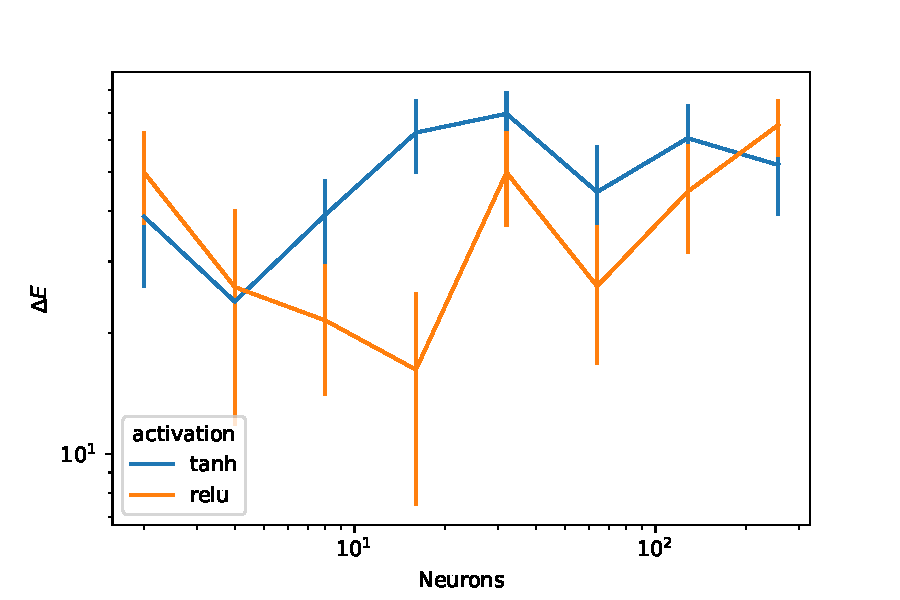
\includegraphics[width=\linewidth]{figures/curve_so3/pl_eks_6/neurons_error.pdf}
        \caption{The final cost \(E\) with the number of neurons in each hidden layer.}\label{fig:curve_so3_pl_neuron_error}
    \end{subfigure}
    \begin{subfigure}[t]{0.5\textwidth}
        \centering
        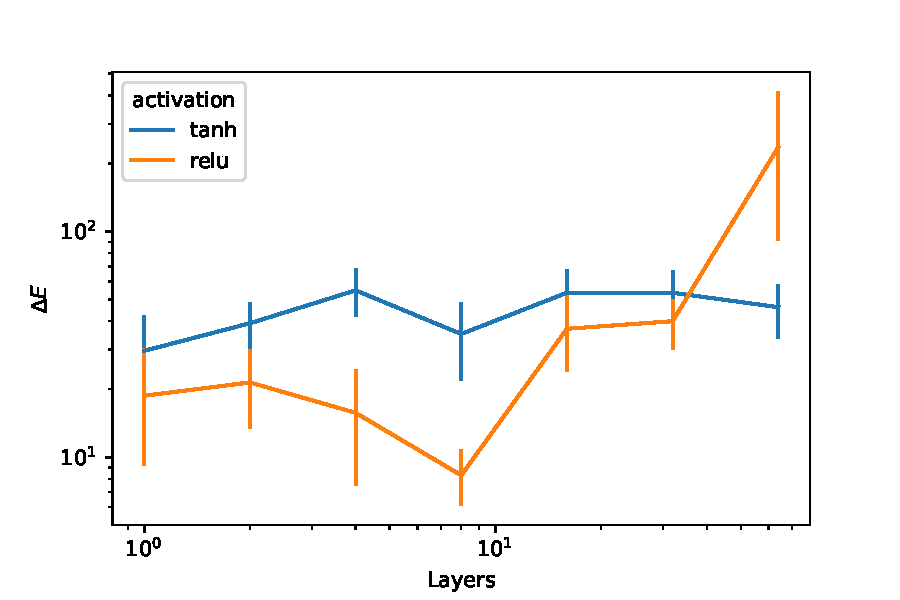
\includegraphics[width=\linewidth]{figures/curve_so3/pl_eks_6/layer_error.pdf}
        \caption{Final cost \(E\) with the number of layers.}\label{fig:curve_so3_pl_layer_error}
    \end{subfigure}
    \caption{Result of ensemble training for the piecewise linear version of the problem with curves generated by motion capture data with different number of neurons and hidden layers. Figure \ref{fig:curve_2_neuron_error} the number of layers was fixed at 2. In Figure \ref{fig:curve_2_layer_error} the number of neurons is fixed at 8 per hidden layer. The error bars denote a 80\% confidence interval found by bootstrapping.}\label{fig:curve_so3_pl_eks}
\end{figure}

